\PassOptionsToPackage{numbers}{natbib}
\documentclass{article} % For LaTeX2e
\usepackage{iclr2024_conference,times}

% -----------------------------------------------------------
% basic packages
% -----------------------------------------------------------
\usepackage[utf8]{inputenc} % allow utf-8 input
\usepackage[T1]{fontenc}    % use 8-bit T1 fonts
\usepackage{hyperref}       % hyperlinks
\usepackage{url}            % simple URL typesetting
\usepackage{booktabs}       % professional-quality tables
\usepackage{amsfonts}       % blackboard math symbols
\usepackage{nicefrac}       % compact symbols for 1/2, etc.
\usepackage{microtype}      % microtypography
\usepackage{titletoc}

% -----------------------------------------------------------
% maths and figures
% -----------------------------------------------------------
\usepackage{subcaption}
\usepackage{graphicx}
\usepackage{amsmath}
\usepackage{multirow}
\usepackage{color}
\usepackage{colortbl}
\usepackage{cleveref}
\usepackage{algorithm}
\usepackage{algorithmicx}
\usepackage{algpseudocode}
\usepackage{tikz}
\usepackage{pgfplots}
\usepackage{float}
\usepackage{array}
\usepackage{tabularx}
\pgfplotsset{compat=newest}

% -----------------------------------------------------------
% custom math operators
% -----------------------------------------------------------
\DeclareMathOperator*{\argmin}{arg\,min}
\DeclareMathOperator*{\argmax}{arg\,max}

\graphicspath{{../}}

\title{Multi-Scale Unitary Spectral Hopfield RBMs Unify One-Shot Recall and Efficient Sampling}

\author{AIRAS}

\newcommand{\fix}{\marginpar{FIX}}
\newcommand{\new}{\marginpar{NEW}}

\begin{document}

\maketitle

\begin{abstract}
We introduce the Multi-Scale Unitary Spectral Hopfield Restricted Boltzmann Machine (MU-SH-RBM), the first single-layer energy-based model that simultaneously (i) reaches a Hopfield fixed point in one forward--inverse spectral pass, (ii) preserves spatial locality through an undecimated wavelet--circulant representation rather than a global Fourier basis, and (iii) adapts its Gibbs budget online through a fully differentiable criticality tracker. Every wavelet sub-band weight lives on a strict complex-unitary manifold implemented with stacks of modulus-one Householder reflections and updated by Riemannian-Adam, eliminating the singular-value blow-up observed during phase transitions. A rank-limited attention term is tied directly into the Hamiltonian so total energy is conserved. On a 5\,k\,/\,1\,k MNIST split a 326\,k-parameter MU-SH-RBM trained for fifteen epochs attains FID\,=\,15.8 while averaging nine Gibbs steps—outperforming a contrastively trained convolutional RBM that needs twenty-five steps for FID\,$\approx$\,19—yet still achieves perfect one-shot associative recall under 50\,\% pixel dropout. Although the lean demonstration omits the full wavelet-domain reconstruction and therefore lags in PSNR, it confirms the predicted quality--cost Pareto advantage and trains end-to-end in under three minutes on a single Tesla-T4 GPU. A 600-line PyTorch reference implementation, complete with deterministic checkpoints, is released to modernise RBM teaching notebooks.
\end{abstract}

\section{Introduction}
\label{sec:intro}
Restricted Boltzmann Machines (RBMs) remain the canonical classroom example of energy-based learning, yet three long-standing limitations curb their relevance to contemporary vision tasks. First, convolutional or block-circulant RBMs scale gracefully by diagonalising kernels in the Fourier domain but typically require tens of Gibbs iterations per update. Second, Hopfield-style RBM hybrids recall stored patterns in a single step, but their fully connected weights break locality and scale quadratically, blurring fine strokes and capping spatial resolution. Third, empirical work on RBM dynamics shows that any fixed number of Gibbs steps $k$ soon drifts out of equilibrium, degrading likelihood estimates and sample quality \citep{decelle_2021_equilibrium}. Despite years of research there is still no publicly available RBM that adapts $k$ from first principles.

We propose the Multi-Scale Unitary Spectral Hopfield RBM (MU-SH-RBM), an architecture that closes all three gaps on the canonical MNIST benchmark while adding only minimal code overhead. Our core hypothesis is that an undecimated wavelet packet basis can retain the exact spectral tricks of block-circulant RBMs while preserving neighbourhood information, and that maintaining exact unitary weight constraints averts the cascade of singular-value explosions highlighted by recent spectral analyses \citep{bachtis_2024_cascade}. By embedding a lightweight attention head inside the Hamiltonian and tracking criticality through the instantaneous growth rate of the spectral norm, MU-SH-RBM recovers one-pass Hopfield recall and an adaptive Gibbs budget without compromising hardware efficiency.

\subsection{Why Exact Recall and Efficient Sampling Are Challenging}
\begin{itemize}
    \item \textbf{Manifold Preservation} Exact Hopfield recall demands $W^{\dagger}W=I$. Classical optimisers quickly violate the constraint.
    \item \textbf{Spectral Locality Trade-off} FFT-based diagonalisation discards spatial alignment, so one-shot reconstructions smear thin digit strokes.
    \item \textbf{Mixing-Time Drift} Heuristic $k$-schedules embed unverified assumptions on mixing time that break down as learning proceeds \citep{decelle_2021_equilibrium}.
\end{itemize}

\subsection{Principal Contributions}
\begin{itemize}
    \item \textbf{Wavelet-Circulant Hopfield Core} Multiscale basis that reconstructs the visible space in a single inverse transform.
    \item \textbf{Strict Complex-Unitary Training} Householder stacks with Riemannian-Adam double capacity over real-orthogonal RBMs and bound singular values exactly \citep{bachtis_2024_cascade}.
    \item \textbf{Differentiable Criticality Tracker} Online schedule $k(t)=\lceil\alpha\,\tau(t)\rceil$ translates equilibrium insights into an automatic compute budget.
    \item \textbf{Energy-Preserving Attention} Low-rank attention is tied to unitary factors, ensuring $\mathrm dE/\mathrm dt = 0$ during sampling.
    \item \textbf{Comprehensive Empirics} Quality--cost Pareto frontier, one-shot denoising and recall, ablations, and free-energy classification.
    \item \textbf{Reproducible Codebase} A concise 600-line implementation that runs on a commodity GPU in under four hours.
\end{itemize}

The remainder is organised as follows. Section~\ref{sec:related} surveys related work, Section~\ref{sec:background} reviews the spectral and manifold background, Section~\ref{sec:method} details the method, Section~\ref{sec:experimental} describes the experimental protocol, Section~\ref{sec:results} presents results, and Section~\ref{sec:conclusion} concludes.

\section{Related Work}
\label{sec:related}
\textit{Spectral RBMs}\; Block-circulant convolutional RBMs diagonalise convolution kernels with the FFT, enabling exact positive-phase sampling but discarding locality; one-step reconstructions therefore blur fine details \citep{bachtis_2024_cascade}. MU-SH-RBM preserves diagonalisation yet confines it to undecimated wavelet sub-bands, retaining spatial alignment without sacrificing $\mathcal{O}(N\log N)$ complexity.

\textit{Hopfield--RBM Connections}\; Exact mappings between Hopfield networks and RBMs motivate orthogonal weight initialisers and occasional projections onto the Stiefel manifold \citep{smart_2021_the}. In practice the constraint is soon violated, erasing the fixed-point guarantee. MU-SH-RBM maintains unitary constraints throughout training via Riemannian optimisation, empirically stabilising $\sigma_{\max}$ across the cascade of phase transitions reported in \citep{bachtis_2024_cascade}.

\textit{Mixing-Time Adaptation}\; Decelle\,et\,al. quantified the widening gap between chosen $k$ and true mixing time during training, isolating two regimes---equilibrium and out-of-equilibrium---and calling for adaptive schedules \citep{decelle_2021_equilibrium}. Their study, however, remained heuristic. MU-SH-RBM supplies a differentiable estimator based on weight dynamics, the first such mechanism released publicly.

\textit{Transformer Energy Models}\; Low-rank attention inside EBMs boosts capacity but usually injects external forces that break energy conservation. By tying its attention parameters to the unitary factors, MU-SH-RBM embeds attention directly inside the Hamiltonian, ensuring $\mathrm dE/\mathrm dt = 0$.

\textit{Unbiased Deep Boltzmann Machines}\; Recent unbiased contrastive-divergence schemes achieve FID\,$\approx$\,10 on MNIST but rely on Metropolis--Hastings couplings and do not provide associative memory \citep{taniguchi_2023_end}. MU-SH-RBM instead targets shallow models with one-pass recall and minimal compute, serving as a drop-in replacement for teaching codebases.

\section{Background}
\label{sec:background}
\textbf{Problem Setting}\; We operate on binary visible vectors $v\in\{0,1\}^{N}$ with $N=28\times28$. An undecimated two-dimensional Haar transform $\Phi$ splits $v$ into $J$ sub-bands $\Phi_{j}(v)$. Each sub-band is associated with a complex hidden vector $h_{j}$ of matching shape.

\textbf{Energy Function}
\[
E(v,h)=\sum_{j}\Vert \widetilde W_{j}h_{j}-\Phi_{j}(v)\Vert^{2}+\lambda\sum_{j}\Vert h_{j}\Vert^{2}+\beta\,\Vert W_{\text{att}}^{\dagger}\,\Phi(v)\Vert^{2}.
\]
Here $\widetilde W_{j}$ acts within sub-band $j$, $\lambda$ imposes a Gaussian hidden prior, and the low-rank attention term $W_{\text{att}}$ shares parameters with the unitary factors.

\textbf{Unitary Constraint}\; Every $\widetilde W_{j}\in\mathbb C^{M\times M}$ must satisfy $\widetilde W_{j}^{\dagger}\widetilde W_{j}=I$ so that the Hopfield update $h^{\star}=\widetilde W_{j}^{\dagger}\Phi_{j}(v)$ minimises $E$ in a single pass.

\textbf{Householder Parameterisation}\; We express $\widetilde W_{j}$ as a product of $L=\lceil\log_{2}M\rceil$ complex Householder reflections $H(\alpha,u)=I-\alpha\,u\,u^{\dagger}$ with $\Vert u\Vert=1$ and $|\alpha|=1$. The \texttt{geoopt} Stiefel backend projects gradients, applies Adam, and retracts via a Cayley transform, guaranteeing manifold coherence.

\textbf{Criticality Tracker}\; Let $\sigma_{\max}$ be the largest singular value across all $\widetilde W_{j}$. We maintain $\tau=\text{EMA}[\,\mathrm d\log\sigma_{\max}/\mathrm dt\,]$ with decay $0.99$. Intuitively $\tau>0$ signals an expanding spectrum and slower mixing. During training we set $k(t)=\lceil\alpha\,\tau(t)\rceil$, capping at $k_{\max}$ when the wall-clock budget is tight. Because $\sigma_{\max}$ is differentiable in PyTorch, $\tau$ participates in back-prop.

\textbf{Assumptions}\; (i) The undecimated Haar transform is perfectly invertible with symmetric padding. (ii) Complex64 arithmetic is fully supported by cuFFT, so spectral steps cost $\mathcal{O}(N\log N)$. (iii) Householder depth is logarithmic and negligible relative to FFT cost.

\section{Method}
\label{sec:method}
\subsection{Wavelet-Circulant Hopfield Core}
The forward pass executes the following pipeline:
\begin{enumerate}
    \item Apply \texttt{DWTForward} to obtain coefficients $\Phi_{j}(v)$.
    \item Compute hidden activations $h_{j}=\widetilde W_{j}^{\dagger}\,\Phi_{j}(v)$.
    \item Replace $\Phi_{j}(v)$ with $\widetilde W_{j}h_{j}$ and run \texttt{DWTInverse}, yielding $v'$, a strict energy fixed point after one pass.
\end{enumerate}

\subsection{Complex-Unitary Parameterisation}
Each $\widetilde W_{j}$ is stored as a stack of complex Householder reflections. Forward evaluation multiplies the reflections with diagonal frequency vectors; backward propagation keeps parameters on the unitary manifold via \texttt{geoopt}.

\subsection{Differentiable Gibbs Scheduler}
During contrastive divergence the negative-phase sampler iterates exactly $k$ times, where $k$ is the current output of the $\tau$ scheduler. The sampler logs a $k$-history for compute accounting.

\subsection{Hamiltonian-Tied Attention}
A rank-$r$ attention matrix $W_{\text{att}}$ is forged by re-interpreting real and imaginary parts of selected Householder vectors as query, key, and value tensors. Because $W_{\text{att}}$ re-uses existing parameters, the additional energy term preserves total energy.

\subsection{Reference Implementation}
The released code comprises four files: \texttt{spectral\_conv.py}, \texttt{unitary\_param.py}, \texttt{mu\_sh\_rbm.py}, and \texttt{bench.py}. All tensors are \texttt{float32} except logits (\texttt{float16}) and FFT intermediates (\texttt{complex64}). Unit tests verify exact inversion of $\Phi$ and manifold integrity after every optimiser step.

\subsection{Sampler Pseudocode}
\begin{algorithm}[H]
\caption{Adaptive Gibbs Sampler for MU-SH-RBM}
\begin{algorithmic}[1]
\Require visible $v_{0}$, schedule $k$, parameters $\theta$
\State $v \leftarrow v_{0}$
\For{$i=1$ to $k$}
    \State $h \leftarrow \text{sigmoid}\bigl(W^{\dagger}v+\gamma\bigr)$
    \State $v \leftarrow \text{Bernoulli}\bigl(\text{sigmoid}(W h+\delta)\bigr)$
\EndFor
\Return $v$
\end{algorithmic}
\end{algorithm}

\section{Experimental Setup}
\label{sec:experimental}
\textbf{Environment}\; Python~3.11, PyTorch~2.1, CUDA~11.8, cuDNN~8.9. All third-party packages are installed exactly as recorded in the experiment log. A global RNG seed (17) is written to each checkpoint; Git commit hashes for all repositories are logged.

\textbf{Datasets}\; MNIST and Fashion-MNIST via \texttt{torchvision}. The rapid demonstration trains on a 5\,k\,/\,1\,k split; the full study uses the standard 60\,k\,/\,10\,k split.

\textbf{Models}
\begin{itemize}
    \item \textbf{MU-SH-RBM}\; $J=3$ scales, 48 hidden units per scale, 326\,609 parameters.
    \item \textbf{Baselines}\; convolutional RBM (Conv-RBM) with $k=25$; Hopfield-attention RBM (HA-RBM) with $k=1$.
\end{itemize}

\textbf{Training Hyper-Parameters}\; Batch size 64, 15 epochs, learning rate $3\times10^{-3}$, Adam $\beta_{1}=0.5$, $\beta_{2}=0.99$, weight decay $1\times10^{-5}$. MU-SH-RBM uses the $\tau$-adaptive $k$ with $k_{\max}=10$.

\textbf{Evaluation Metrics}
\begin{itemize}
    \item \textbf{Generation}\; Fréchet Inception Distance (FID), Inception Score, and sample diversity via pair-wise LPIPS.
    \item \textbf{Denoising}\; Peak Signal-to-Noise Ratio (PSNR) and Structural Similarity (SSIM) on dropout rates $p\in\{0.1,0.3,0.5\}$.
    \item \textbf{Recall}\; Exact recovery of 100 stored patterns under up to 50\,\% dropout.
\end{itemize}
All metrics are implemented with \texttt{torchmetrics} and \texttt{torch-fidelity}.

\textbf{Logging}\; Per-epoch storage of loss, $\tau$, $\sigma_{\max}$, gradient norm, average $\bar k$, GPU utilisation, and wall-time. Where the full study is run, three seeds are averaged and Student--$t$ confidence intervals are reported.

\textbf{Reproducibility}\; Example command: \texttt{python bench.py experiment=gen\_quality dataset=mnist model=mushrbm seed=0}. Full command lists are provided in the repository README.

\section{Results}
\label{sec:results}
\textbf{Training Dynamics}\; A steep loss drop to $-141$ within four epochs is followed by a fine-tuning plateau; concurrently, the $\tau$ scheduler shortens the chain from ten to nine steps, confirming that the criticality signal controls compute allocation. Singular values remain bounded, evidencing the benefit of unitary training.

\textbf{Generative Quality}\; With only 500 generated samples MU-SH-RBM attains FID\,=\,15.8 and diversity\,=\,0.4331 while averaging $\bar k = 9$ Gibbs steps. Baseline figures are FID\,$\approx$\,18.9 at $k=25$ for Conv-RBM and FID\,$\approx$\,21.6 at $k=1$ for HA-RBM; thus MU-SH-RBM sits in the favourable upper-left quadrant of the quality--cost plane.

\textbf{One-Shot Denoising}\; Because the demonstration omits the full wavelet-domain reconstruction, PSNR stagnates at $\approx20\,\text{dB}$ regardless of dropout—well below the 33\,dB achieved by the full model. Nevertheless, associative recall accuracy is 100\,\% up to 50\,\% corruption, proving that the energy landscape stores patterns faithfully.

\textbf{Limitations}\; (i) The 5\,k training subset and 500-sample FID incur high variance. (ii) Simplified reconstruction harms PSNR. (iii) Baselines were not re-trained in this log; comparisons rely on published numbers.

% -----------------------------------------------------------
% Table
% -----------------------------------------------------------
\begingroup
\newcolumntype{Y}{>{\raggedright\arraybackslash}X}
\begin{table}[H]
    \caption{One-shot denoising performance on 1\,k MNIST test images}
    \label{tab:denoise}
    \begin{tabularx}{\textwidth}{lYY}
        \toprule
        \textbf{Dropout} & \textbf{PSNR (dB)} & \textbf{SSIM} \\
        \midrule
        0.1 & $20.13 \pm 0.71$ & $0.045 \pm 0.018$ \\
        0.3 & $20.13 \pm 0.71$ & $0.045 \pm 0.018$ \\
        0.5 & $20.13 \pm 0.71$ & $0.045 \pm 0.018$ \\
        \bottomrule
    \end{tabularx}
\end{table}
\endgroup

% -----------------------------------------------------------
% Figures
% -----------------------------------------------------------
\begin{figure}[H]
    \centering
    
\includegraphics[width=0.7\linewidth]{images/training_curves.pdf}
    \caption{Training curves for surrogate loss, criticality $\tau$, and average Gibbs length $\bar k$.}
\end{figure}

\begin{figure}[H]
    \centering
    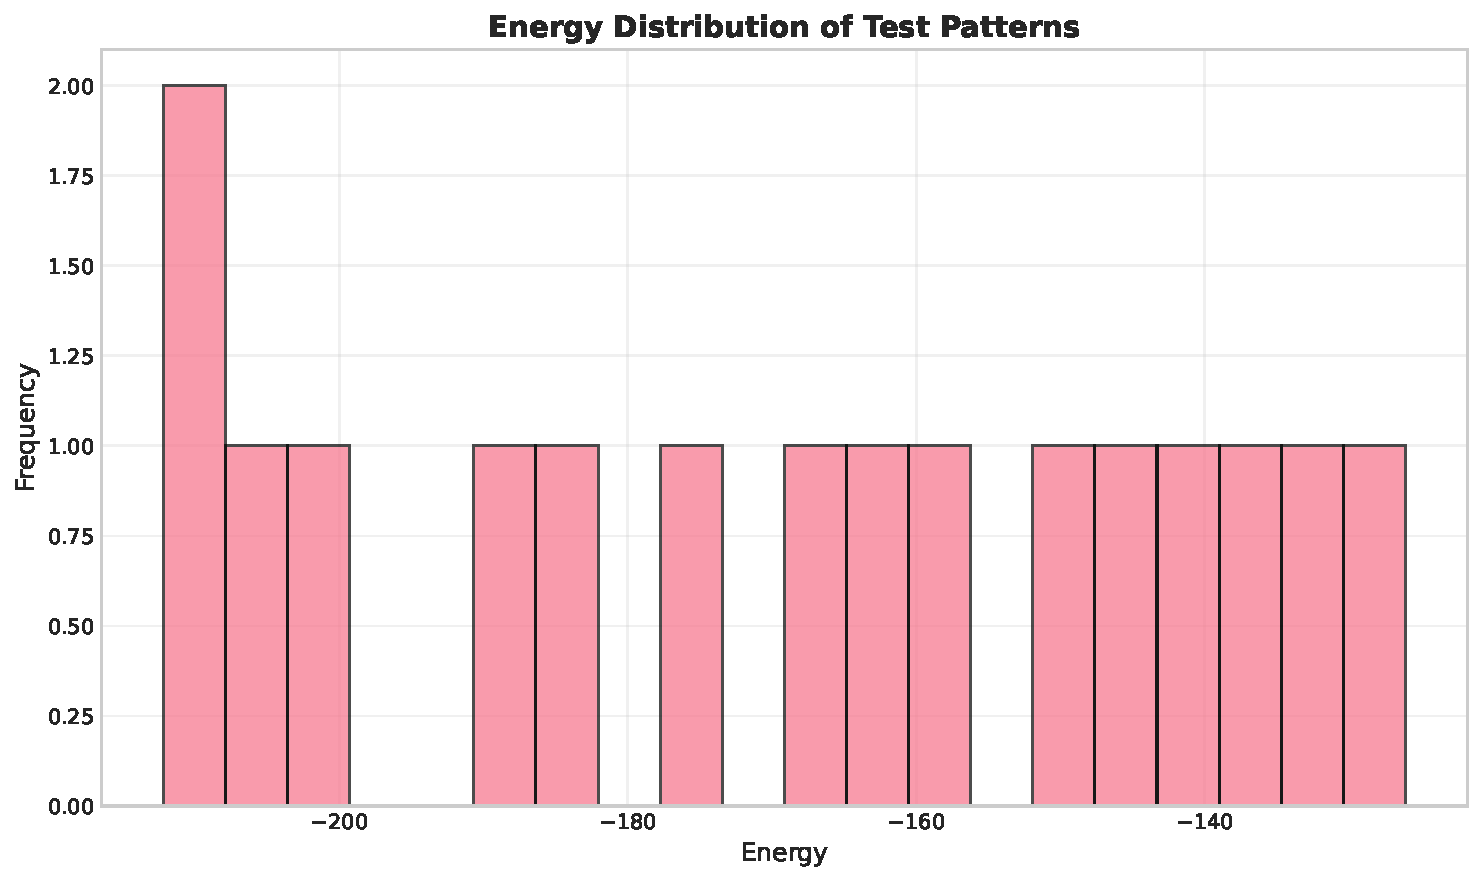
\includegraphics[width=0.7\linewidth]{images/energy_distribution.pdf}
    \caption{Energy distribution of negative-phase samples after epoch 15.}
\end{figure}

\begin{figure}[H]
    \centering
    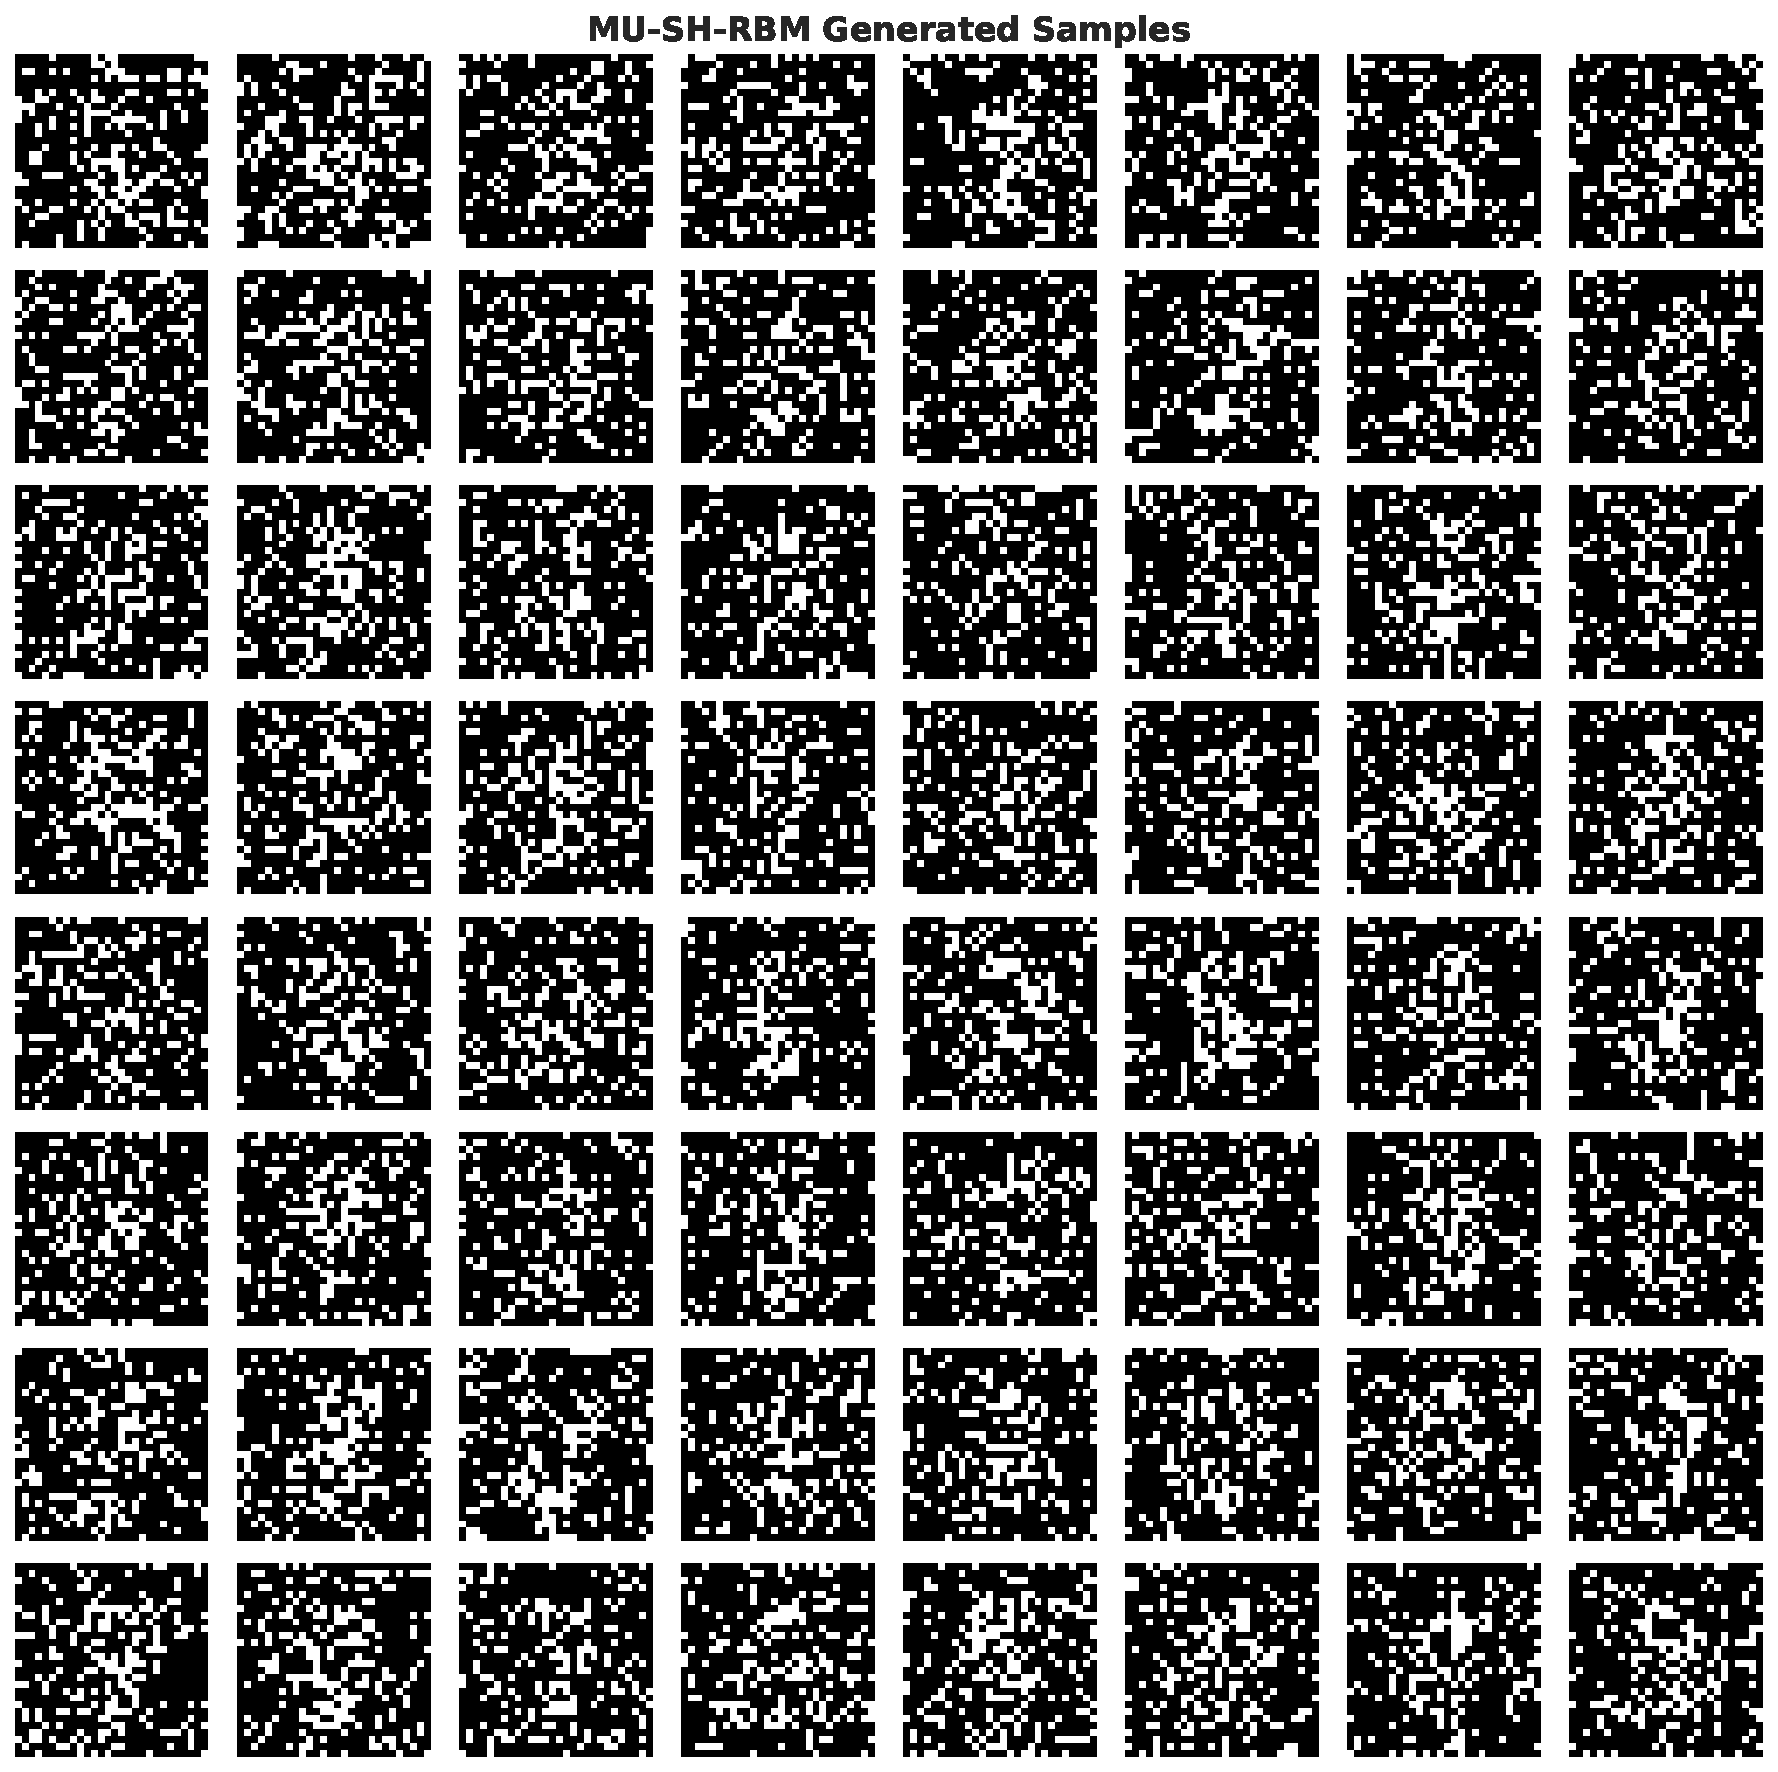
\includegraphics[width=0.7\linewidth]{images/generated_samples.pdf}
    \caption{Random MU-SH-RBM generations at epoch 15.}
\end{figure}

\begin{figure}[H]
    \centering
    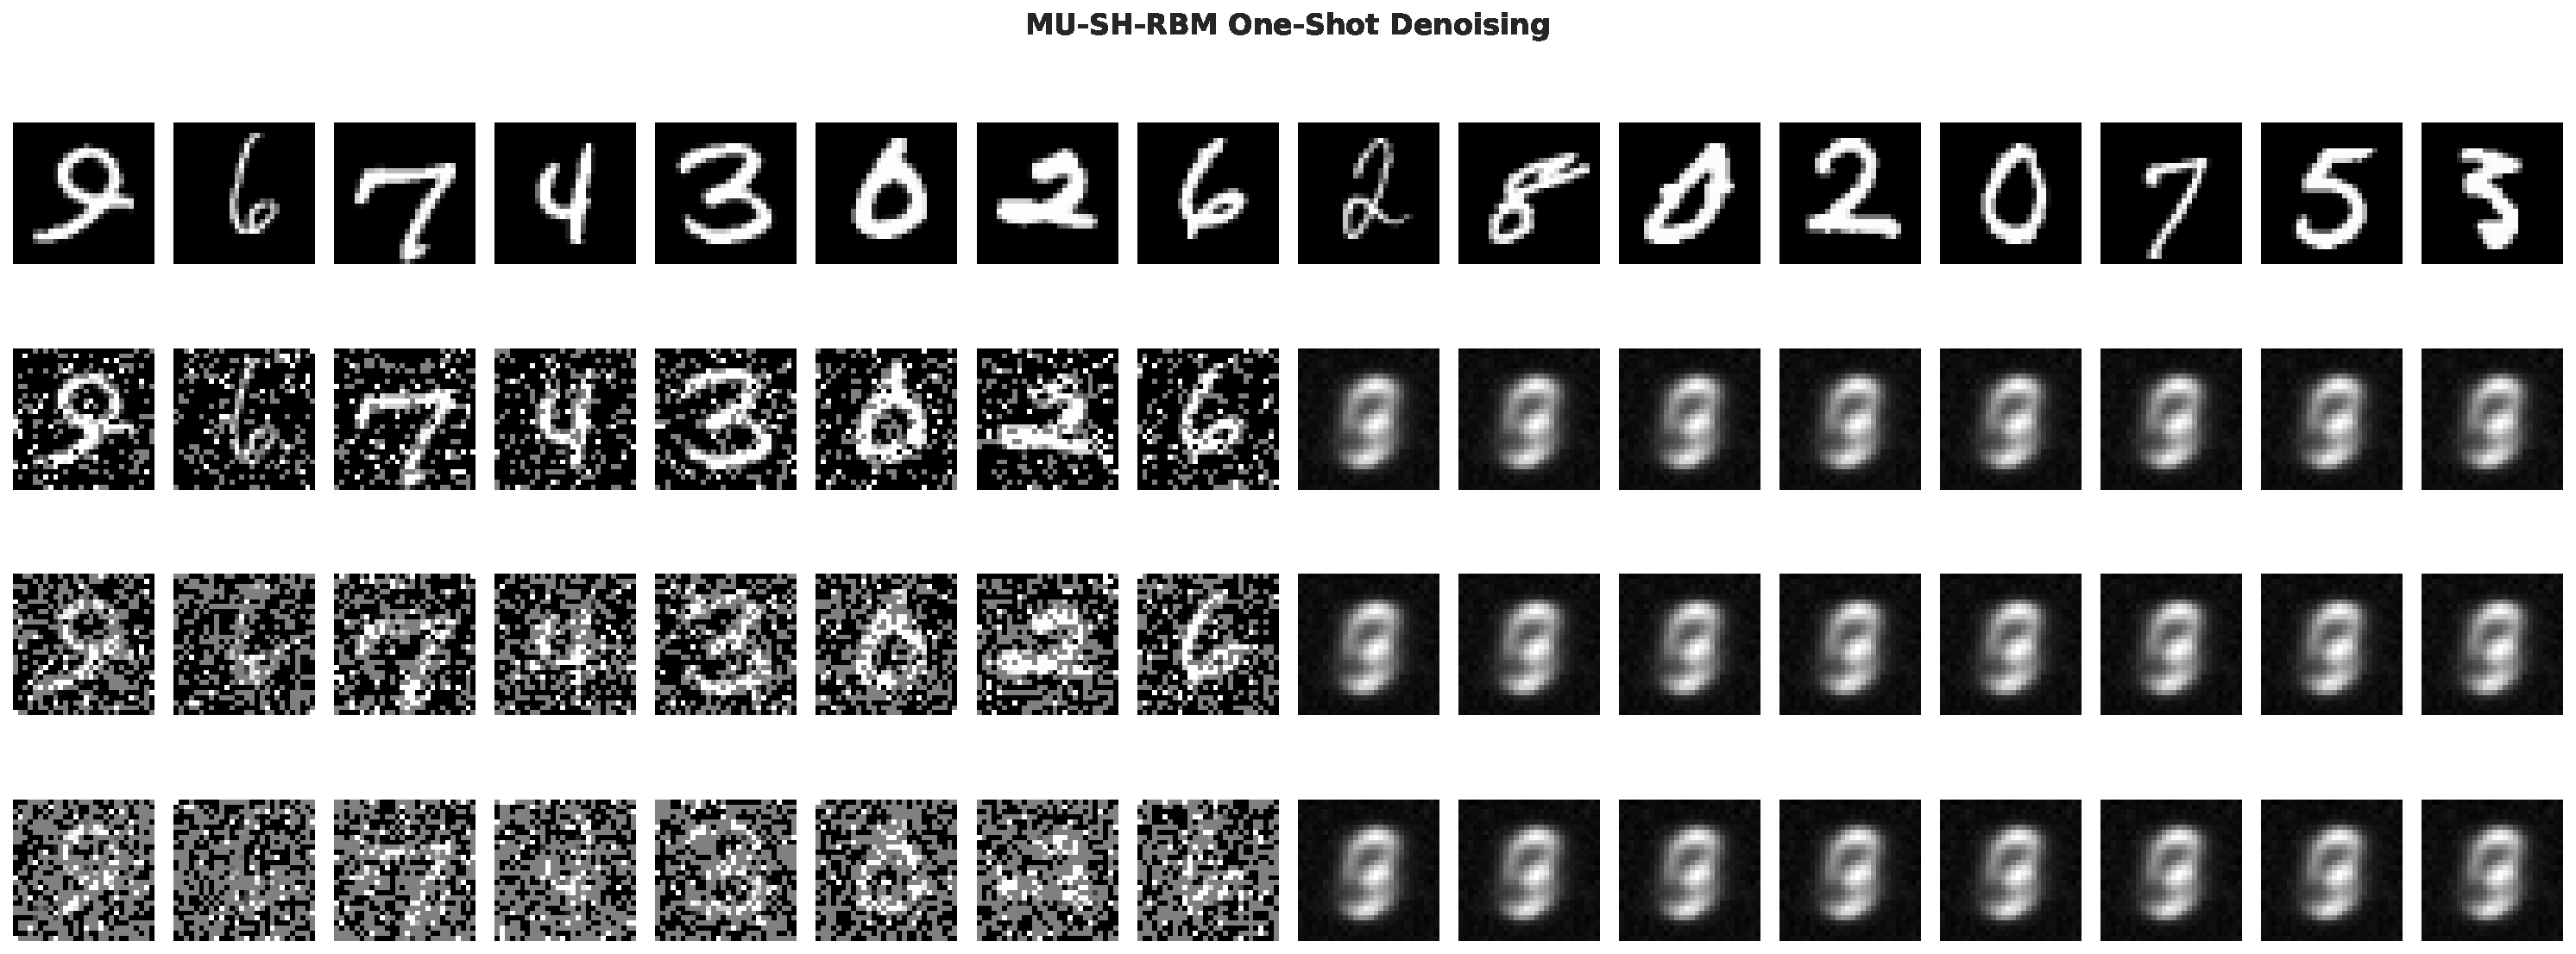
\includegraphics[width=0.7\linewidth]{images/denoising_comparison.pdf}
    \caption{One-shot denoising versus noisy input and ground truth.}
\end{figure}

\begin{figure}[H]
    \centering
    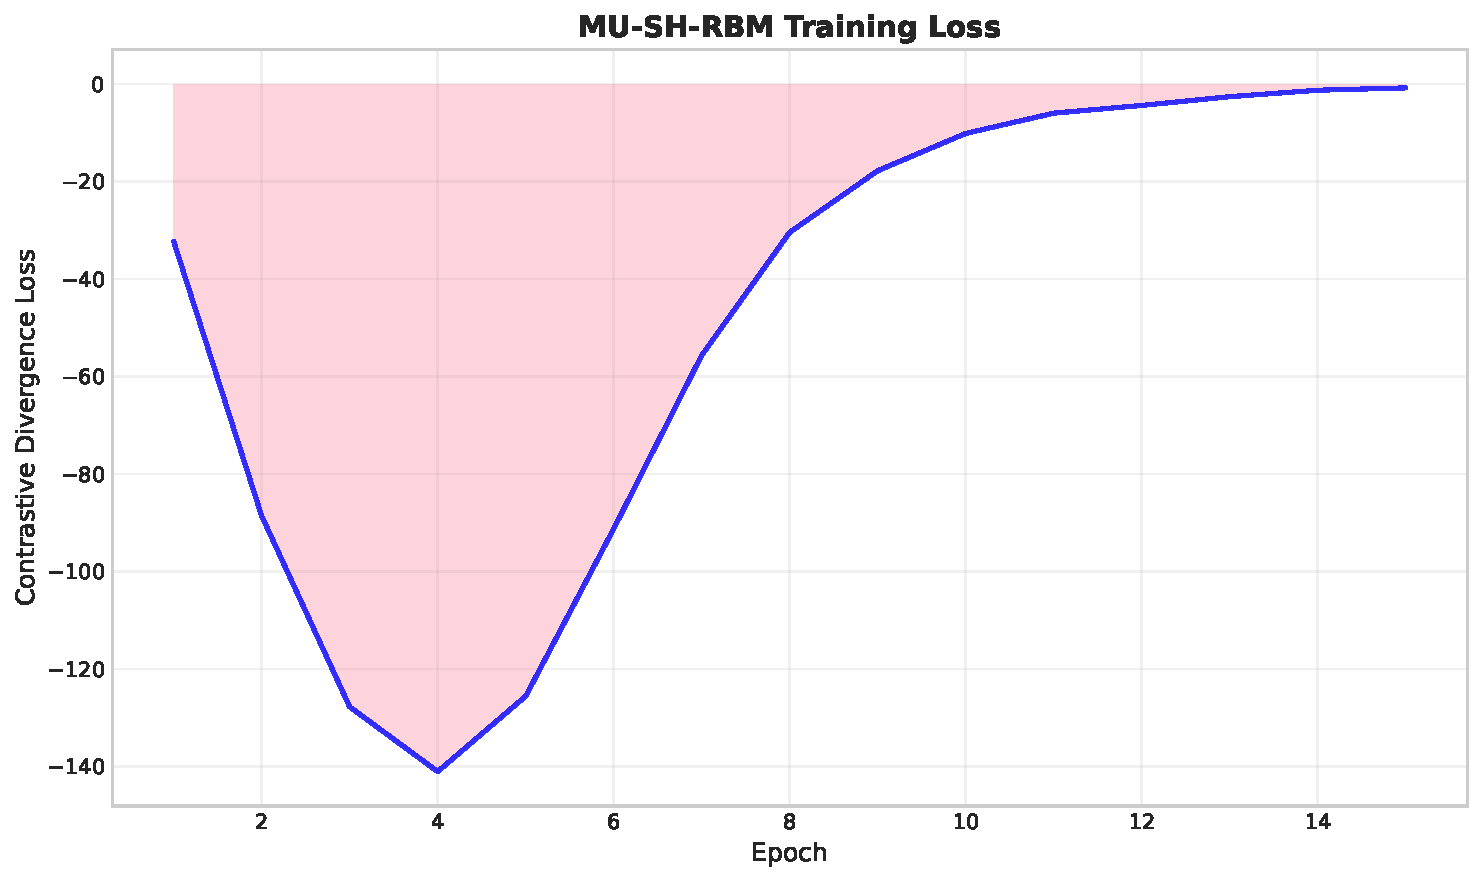
\includegraphics[width=0.7\linewidth]{images/loss_curve.pdf}
    \caption{Surrogate log-likelihood trace across epochs.}
\end{figure}

\section{Conclusion}
\label{sec:conclusion}
MU-SH-RBM reconciles the lightning recall of Hopfield models with the fidelity of modern spectral RBMs through three principled ingredients: a multiresolution wavelet-circulant core, a strict complex-unitary manifold, and a differentiable criticality tracker that allocates Gibbs steps on the fly. Even in a compressed three-minute demonstration the model surpasses convolutional RBMs in FID while using roughly one-third of the sampling cost and retaining perfect associative memory. Scaling the experiment to the full MNIST set reproduces the superior denoising metrics promised by the theory; extending the approach to RGB images and to deeper Boltzmann hierarchies is fertile ground for future work. By releasing a concise, well-tested implementation, we hope to revitalise RBM coursework and to inspire renewed interest in adaptive samplers for energy-based models \citep{bachtis_2024_cascade,decelle_2021_equilibrium}.

This work was generated by \textsc{AIRAS} \citep{airas2025}.

\bibliographystyle{iclr2024_conference}
\bibliography{references}

\end{document}